%%%%%%%%%%%%
%
% $Autor: Adhiraj $
% $Datum: 2024-12-25 08:03:15Z $
% $Pfad: TemplateSensor $
% $Version: 4250 $
% !TeX spellcheck = en_GB/de_DE
% !TeX encoding = utf8
% !TeX root = Algorithm 
% !TeX TXS-program:bibliography = txs:///biber
%
%%%%%%%%%%%%


\chapter{Convolutional Neural Networks(CNN)}

\section{Introduction}

Recent advancements in artificial intelligence, particularly in deep learning, have significantly impacted various cutting-edge technology applications, ranging from autonomous vehicles to creative fields like music and art generation. A central ambition within the scientific community is to enable computers to communicate and comprehend language in a manner akin to human interaction \cite{Li:2021}. As a subset of machine learning, deep learning stands out due to its focus on learning data representations rather than relying on predefined task-specific algorithms. This methodology empowers systems to build complex concepts by integrating information from simpler, fundamental elements.

A Convolutional Neural Network (CNN) has been selected to develop the model, building upon and enhancing the ideas proposed by Warden and Giménez \cite{Warden:2020}. This choice makes CNN an ideal candidate for applications in voice recognition.

Convolutional Neural Networks (CNNs) are a specialized type of multi-layer neural network designed to identify visual patterns in images directly with minimal preprocessing. In artificial neural networks, a neuron serves as a transformative unit that processes inputs to produce outputs. The number of neurons utilized varies based on the specific task and can range from a few to several thousand. Artificial neurons are interconnected in various configurations to form a CNN. Within this structure, individual neurons receive inputs from others, with each input's weight determining its positive or negative influence. 

The collective learning of the network enables it to perform critical computations required for tasks like object recognition and language understanding. These interconnected neurons form a feed-forward network, where outputs from one layer are passed to subsequent layers. This process continues until a final output is generated \cite{Gu:2018}.


\section{Description}

Understanding the internal mechanisms of the model is not essential for its application; however, exploring these processes can be valuable for addressing potential issues and is intrinsically engaging. This section provides an overview of the model's predictive functionality. Within neural network architecture, a specific type excels in managing multidimensional tensors by leveraging the relationships between neighboring values—known as a Convolutional Neural Network (CNN). Although typically used for image processing, where inputs are 2D pixel grids, CNNs demonstrate exceptional adaptability in analyzing spectrogram data, highlighting their utility beyond traditional visual tasks \cite{Warden:2020}.
This section introduces the basic concepts of CNN. Furthermore, descriptions of crucial elements including the optimizer, loss function, and activation function.

\subsection{CNN Components}

Convolutional Neural Networks (CNNs) are a type of feedforward neural network that excel in automatically extracting features from data through their convolutional architecture. Unlike traditional methods that rely on manual feature extraction, CNNs streamline this process by learning features directly from the data. Inspired by visual perception, CNNs employ kernels that act as artificial receptors, detecting various features and aligning artificial neurons with the behavior of biological neurons. 

Activation functions, analogous to the biological threshold for signal transmission, simulate the electrical signaling between neurons. Meanwhile, loss functions and optimizers play a critical role in guiding the CNN to identify and learn the desired patterns effectively \cite{Li:2021}.

Compared to fully connected (FC) networks (see Figure \ref{fig:CNNandFCLayers}), CNNs offer several advantages:

\begin{itemize}
	\item \textbf{Localized Connections:} In CNNs, neurons connect only to a subset of the previous layer rather than all neurons, reducing parameters and computational complexity. This structure helps focus on spatially relevant features and speeds up convergence.
	\item \textbf{Weight Sharing:} A single set of weights is reused across different locations in the input, capturing patterns like edges regardless of position. This reduces parameters and improves generalization.
	\item \textbf{Downsampling:} Pooling layers summarize data by retaining key features (e.g., max or average values), reducing spatial dimensions and computational cost while eliminating redundant information.
\end{itemize}


\begin{figure}[h!]
	\centering
	\includegraphics[width=0.8\textwidth]{Images/Algorithm/CNNandFCLayers}
	\caption{CNN and FC layers \cite{Wings:2023}} \label{fig:CNNandFCLayers}
\end{figure}


Convolution is a key step in the feature extraction process, generating feature maps. Padding, achieved by adding zero values to the input, helps prevent information loss at the edges of the input. Stride controls the density of the convolution operation. However, the feature maps produced can lead to overfitting, necessitating the use of pooling (either max pooling or average pooling) to eliminate redundant information. Figure \ref{fig:ProcedureCNN} illustrates the overall CNN workflow. Below is a detailed explanation of padding, stride, and pooling \cite{Li:2021}:

\begin{itemize}
	\item \textbf{Padding:} Padding refers to the addition of extra pixels around the edges of the input image before the convolution process. This is typically done by surrounding the image with rows and columns filled with zeros. The purpose of padding is to prevent the loss of information at the image borders during convolution.
	
	\item \textbf{Stride:} Stride refers to the step size, or the number of pixels the convolution filter moves across the image during the convolution operation. A larger stride results in smaller feature maps, which leads to a more compact representation.
	
	\item \textbf{Pooling:} Pooling is a down-sampling technique applied after convolution that reduces the size of the feature maps. It helps control the number of parameters in the network. Common pooling methods include max pooling and average pooling \cite{Wings:2023}.
	
	\begin{enumerate}
		\item \textbf{Max Pooling:} Max pooling is a pooling operation where, for each region of the feature map, the highest value is selected. This preserves the most important features from that region, providing a compact summary of the spatial information.
		
		\item \textbf{Average Pooling:} Average pooling is another pooling method where the average value of each region in the feature map is computed. This technique reduces the spatial dimensions while preserving a smoother, less detailed version of the features.
	\end{enumerate}
\end{itemize}

\begin{figure}[h!]
	\centering
	\includegraphics[width=0.8\textwidth]{Images/Algorithm/ProcedureCNN}
	\caption{Procedure of a two-dimensional CNN} \label{fig:ProcedureCNN}
\end{figure}

The field of Convolutional Neural Networks (CNNs) includes numerous architectural variations, but their fundamental components remain consistent. For instance, the well-known LeNet-5 architecture consists of three primary layers: convolutional, pooling, and fully-connected layers \cite{Gu:2018}. The primary role of the convolutional layer is to extract meaningful feature representations from the input data.

As illustrated in Figure \ref{subfig:LetNet5ArchitectureNetwork}, the convolutional layer comprises multiple convolutional kernels, each responsible for generating unique feature maps. Each neuron in a feature map is connected to a specific region of neurons in the preceding layer, referred to as its receptive field. The creation of a feature map involves convolving the input data with a learned kernel, followed by applying an element-wise nonlinear activation function. Importantly, each feature map is generated by sharing the kernel across all spatial regions of the input, with multiple distinct kernels utilized to produce the complete set of feature maps.

\begin{figure}[h!]
	\centering
	
	\begin{subfigure}{0.65\textwidth}
		\includegraphics[width=\linewidth]{Images/Algorithm/LetNet5ArchitectureNetwork}
		\caption{LetNet-5 network}    % \caption{} is kept to keep (a), (b), (c) etc. below each subfigure.
		\label{subfig:LetNet5ArchitectureNetwork}
	\end{subfigure}
	\hfill
	\begin{subfigure}{0.3\textwidth}
		\includegraphics[width=\linewidth]{Images/Algorithm/LetNet5ArchitectureLearnedFeatures}
		\caption{Learned features}    % \caption{} is kept to keep (a), (b), (c) etc. below each subfigure.
		\label{subfig:LetNet5ArchitectureLearnedFeatures}
	\end{subfigure}
	
	\caption{The architecture of the LeNet-5 network \cite{Gu:2018}. (\subref{subfig:LetNet5ArchitectureNetwork}) The architecture of the LeNet-5 network, renowned for its effectiveness in digit classification tasks. (\subref{subfig:LetNet5ArchitectureLearnedFeatures}) Displaying the features within the LeNet-5 network through visualizations, where each layer's feature maps are showcased in distinct blocks.}
	\label{fig:LetNet5Architecture}
\end{figure}

Mathematically, the feature value at location $(i, j)$ in the $k$th feature map of the $l$th layer (denoted as $z^l_{i,j,k}$) is computed by the expression:

\begin{equation}
	z^l_{i,j,k} = {\mathbf{w}^l_k}^T \mathbf{x}^l_{i,j} + b^l_k
\end{equation}

Here, $\mathbf{w}^l_k$ and $b^l_k$ denote the weight vector and bias term of the $k$th filter in the $l$th layer, respectively, while $\mathbf{x}^l_{i,j}$ represents the input patch centered at location $(i, j)$ in the $l$th layer. The weight-sharing mechanism, where the same kernel is used to generate the feature map across the input, helps reduce model complexity and improves the efficiency of network training.

The activation function ($a(\cdot)$) introduces nonlinearity into the CNN, which is essential for detecting complex, nonlinear patterns in multi-layer networks. The activation value ($a_{l,i,j,k}$) of the convolutional feature $z_{l,i,j,k}$ is calculated as:

\begin{equation}
	a^l_{i,j,k} = a(z^l_{i,j,k})
\end{equation}

Common activation functions include sigmoid, tanh, and ReLU.The pooling layer, positioned between convolutional layers, aims to achieve shift-invariance by downsampling the feature maps' resolution. Each feature map in the pooling layer connects to its corresponding feature map in the preceding convolutional layer. The pooling operation, denoted as $\mathrm{pool}(\cdot)$, is applied to each feature map $a^l_{m,n,k}$ with:

\begin{equation}
	y^l_{i,j,k} = \mathrm{pool}(a^l_{m,n,k}), \forall (m, n) \in \mathcal{R}_{ij}
\end{equation}

In this context, $\mathcal{R}_{ij}$ represents a local neighborhood around the location $(i, j)$. Common pooling techniques include average pooling and max pooling. As shown in Figure \ref{subfig:LetNet5ArchitectureLearnedFeatures} for the digit 7, the learned feature maps progressively capture hierarchical patterns. Early layers extract low-level features, such as edges and curves, while deeper layers encode more abstract and high-level representations.

After the convolutional and pooling layers, one or more fully-connected layers are often used for high-level reasoning. These layers establish dense connections by linking all neurons from the previous layer to each neuron in the current layer, generating global semantic representations. A fully-connected layer can also be replaced by a $1 \times 1$ convolutional layer to achieve similar functionality.

The final layer in CNNs serves as the output layer. For classification tasks, the softmax function is frequently used. Alternatively, CNN features can be combined with Support Vector Machines (SVM) to address various classification challenges. Let the desired input-output relationships be represented as $\{(\mathbf{x}^{(n)}, \mathbf{y}^{(n)}); n \in [1, \ldots, N]\}$. The CNN parameters, denoted by $\mathbf{\theta}$ (including weight vectors and bias terms), are optimized by minimizing a task-specific loss function:


\begin{equation}
	\mathcal{L} = \frac{1}{N} \sum_{n=1}^{N} \ell(\mathbf{\theta}; \mathbf{y}^{(n)}, \mathbf{o}^{(n)})
\end{equation}

Here, $\mathcal{L}$ represents the loss function, which quantifies the discrepancy between the predicted output ($\mathbf{o}^{(n)}$) and the actual target label ($\mathbf{y}^{(n)}$) for $n$th input data point $\mathbf{x}^{(n)}$. The symbol $\mathbf{\theta}$ denotes all the parameters of the CNN, including weight vectors and bias terms. The function $\ell(\mathbf{\theta}; \mathbf{y}^{(n)}, \mathbf{o}^{(n)})$ is the individual loss for a specific data point, measuring the dissimilarity between the predicted output and the true label. The goal during training is to minimize the average loss over all data points, achieved through techniques such as stochastic gradient descent.

The training of a CNN involves global optimization, with the aim of finding the best set of parameters by minimizing the loss function. Stochastic gradient descent emerges as a common solution for optimizing CNN networks, providing an effective means of iterative parameter adjustment.  

\subsection{Activation Function}
\label{subsection:ActivationFunction}

Convolutional Neural Networks (CNNs) utilize a variety of activation functions to capture complex features \cite{Li:2021}. Similar to the behavior of neurons in the human brain, the activation function acts as a mechanism that determines whether information is passed to the next neuron. In a multilayer neural network, activation functions are positioned between layers, as shown in Figure \ref{fig:activationFunctionStructure}.

In Figure \ref{fig:activationFunctionStructure}, $x_i$ represents the input features, with $n$ features simultaneously fed into neuron $j$. The term $w_{ij}$ corresponds to the weight of the connection between input feature $x_i$ and neuron $j$, $b_j$ represents the bias (internal state) of neuron $j$, and $y_j$ is the neuron's output. The activation function, denoted as $f(\cdot)$, may include options such as sigmoid, tanh, or rectified linear unit (ReLU), among others.

If no activation function or a linear activation function is applied, the network’s output becomes a simple linear combination of the inputs, which restricts its learning ability. Introducing nonlinear activation functions, such as sigmoid or tanh, enables the network to model and fit more complex patterns in the data.

\begin{figure}[h!]
	\centering
	\includegraphics[width=0.6\textwidth]{Images/Algorithm/activationFunctionStructure}
	\caption{Structure of an activation function \cite{Li:2021}.} \label{fig:activationFunctionStructure}
\end{figure}

Some of the well-known actiovatoion functions are shown in the Figure \ref{fig:activationFunctions}. The sigmoid function maps a real number to (0, 1), suitable for binary classification. The tanh function maps to (-1, 1), aiding normalization. ReLU, with its advantages in learning speed, is preferred in deep networks. Leaky ReLU and PReLU address limitations of ReLU, reducing neuron inactivation. ELU improves convergence by having a negative output average.

Swish, proposed by Google, and mish, a novel activation function, demonstrate improved performance compared to ReLU and Swish in deeper models across diverse datasets. mish, in particular, exhibits superior gradient flow, accuracy, and generalization properties. Experimental results consistently support the effectiveness of Mish across standard architectures.

\begin{figure}[h!]
	\centering
	
	\begin{subfigure}{0.22\textwidth}
		\includegraphics[width=\linewidth]{Images/Algorithm/SigmoidFunction}
		\caption{}    % \caption{} is kept to keep (a), (b), (c) etc. below each subfigure.
		\label{subfig:Sigmoid}
	\end{subfigure}
	\hfill
	\begin{subfigure}{0.22\textwidth}
		\includegraphics[width=\linewidth]{Images/Algorithm/TanhFunction}
		\caption{}    % \caption{} is kept to keep (a), (b), (c) etc. below each subfigure.
		\label{subfig:Tanh}
	\end{subfigure}
	\hfill
	\begin{subfigure}{0.22\textwidth}
		\includegraphics[width=\linewidth]{Images/Algorithm/ReLUFunction}
		\caption{}    % \caption{} is kept to keep (a), (b), (c) etc. below each subfigure.
		\label{subfig:ReLU}
	\end{subfigure}
	\hfill
	\begin{subfigure}{0.22\textwidth}
		\includegraphics[width=\linewidth]{Images/Algorithm/LeakyReLUFunction}
		\caption{}    % \caption{} is kept to keep (a), (b), (c) etc. below each subfigure.
		\label{subfig:LeakyReLU}
	\end{subfigure}
	
	\medskip
	
	\begin{subfigure}{0.22\textwidth}
		\includegraphics[width=\linewidth]{Images/Algorithm/PReLUFunction}
		\caption{}    % \caption{} is kept to keep (a), (b), (c) etc. below each subfigure.
		\label{subfig:PReLU}
	\end{subfigure}
	\hfill
	\begin{subfigure}{0.22\textwidth}
		\includegraphics[width=\linewidth]{Images/Algorithm/ELUFunction}
		\caption{}    % \caption{} is kept to keep (a), (b), (c) etc. below each subfigure.
		\label{subfig:ELU}
	\end{subfigure}
	\hfill
	\begin{subfigure}{0.22\textwidth}
		\includegraphics[width=\linewidth]{Images/Algorithm/SwishFunctions}
		\caption{}    % \caption{} is kept to keep (a), (b), (c) etc. below each subfigure.
		\label{subfig:Swish}
	\end{subfigure}
	\hfill
	\begin{subfigure}{0.22\textwidth}
		\includegraphics[width=\linewidth]{Images/Algorithm/MishFunction}
		\caption{}    % \caption{} is kept to keep (a), (b), (c) etc. below each subfigure.
		\label{subfig:Mish}
	\end{subfigure}
	
	\caption{Diagrams of activation functions \cite{Li:2021}.  (\subref{subfig:Sigmoid}) Sigmoid function.  (\subref{subfig:Tanh}) Tanh function. (\subref{subfig:ReLU}) ReLU function. (\subref{subfig:LeakyReLU}) Leaky ReLU function. (\subref{subfig:PReLU}) PReLU function. (\subref{subfig:ELU}) ELU function.  (\subref{subfig:Swish}) Swish function. (\subref{subfig:Mish}) Mish function.}
	\label{fig:activationFunctions}
\end{figure}

\subsubsection{Guidelines for Activation Function Selection}

Choosing the right activation function is critical for optimizing the performance of a neural network. Below are some general guidelines to assist in selecting an appropriate activation function:

\begin{enumerate}
	\item For \textbf{binary classification} tasks, use the sigmoid function in the output layer, as it effectively maps outputs to probabilities between 0 and 1. For \textbf{multiclass classification}, the softmax function is more suitable as it normalizes outputs into a probability distribution across multiple classes.
	
	\item While the sigmoid and tanh functions are effective for introducing nonlinearity, they may cause \textbf{gradient vanishing problems}, especially in deep networks. To mitigate this, activation functions like ReLU (Rectified Linear Unit) or leaky ReLU are recommended for hidden layers, as they provide faster convergence and avoid saturation.
	
	\item When there is \textbf{uncertainty} about which activation function to use, ReLU or leaky ReLU can serve as reliable starting points, offering simplicity and consistent performance in most scenarios.
	
	\item If a large number of neurons become \textbf{inactive} during training, resulting in the "dying ReLU" problem, consider alternatives such as leaky ReLU, Parametric ReLU (PReLU), or exponential linear unit (ELU). These activation functions ensure that inactive neurons can still contribute to the learning process.
	
	\item To \textbf{speed up training}, set the negative slope of leaky ReLU to a small value like 0.02. This adjustment prevents neurons from becoming entirely inactive and facilitates faster convergence, particularly in challenging optimization landscapes.
\end{enumerate}

\subsubsection{Guidelines for Activation Function Selection}

Choosing the right activation function is critical for optimizing the performance of a neural network. Below are some general guidelines to assist in selecting an appropriate activation function:

\begin{enumerate}
	\item For \textbf{binary classification} tasks, use the sigmoid function in the output layer, as it effectively maps outputs to probabilities between 0 and 1. For \textbf{multiclass classification}, the softmax function is more suitable as it normalizes outputs into a probability distribution across multiple classes.
	
	\item While the sigmoid and tanh functions are effective for introducing nonlinearity, they may cause \textbf{gradient vanishing problems}, especially in deep networks. To mitigate this, activation functions like ReLU (Rectified Linear Unit) or leaky ReLU are recommended for hidden layers, as they provide faster convergence and avoid saturation.
	
	\item When there is \textbf{uncertainty} about which activation function to use, ReLU or leaky ReLU can serve as reliable starting points, offering simplicity and consistent performance in most scenarios.
	
	\item If a large number of neurons become \textbf{inactive} during training, resulting in the "dying ReLU" problem, consider alternatives such as leaky ReLU, Parametric ReLU (PReLU), or exponential linear unit (ELU). These activation functions ensure that inactive neurons can still contribute to the learning process.
	
	\item To \textbf{speed up training}, set the negative slope of leaky ReLU to a small value like 0.02. This adjustment prevents neurons from becoming entirely inactive and facilitates faster convergence, particularly in challenging optimization landscapes.
\end{enumerate}
Here’s the expanded version with added details and the corresponding LaTeX code:

\subsection{Optimizer}
\label{subsection:optimizer}

In CNNs, optimizing nonconvex functions is a critical step, often requiring robust optimizers to efficiently minimize the loss function within a reasonable timeframe \cite{Li:2021}. Nonconvex functions present complex landscapes with multiple local optima, making optimization challenging. These functions lack the convex property, where a line segment connecting any two points lies entirely within the function's domain, complicating the search for a global minimum. Effective optimization is crucial for improving model accuracy and convergence speed.

\subsubsection{Gradient Descent}

Gradient descent is a fundamental technique for training CNNs, with three common variants: batch gradient descent (BGD), stochastic gradient descent (SGD), and mini-batch gradient descent (MBGD).

\begin{itemize}
	\item \textbf{Batch Gradient Descent (BGD):} BGD calculates the average gradient over the entire dataset for each update. While it provides a stable descent direction, it is computationally expensive and impractical for large datasets due to memory constraints.
	\item \textbf{Stochastic Gradient Descent (SGD):} SGD updates the model parameters using a single data sample per iteration, making it suitable for online learning. However, it can result in high variance and oscillatory convergence due to noisy updates.
	\item \textbf{Mini-Batch Gradient Descent (MBGD):} MBGD strikes a balance between BGD and SGD by computing updates using small batches of data. It reduces variance compared to SGD and is computationally efficient, making it a popular choice for modern deep learning tasks.
\end{itemize}

\begin{itemize}
	\item \textbf{Gradient Descent Optimization Algorithms}
	
	Several advanced algorithms based on MBGD have been developed to address its limitations:
	
	\begin{itemize}
		\item \textbf{Momentum:} Introduces a velocity term to accelerate convergence and reduce oscillations in the optimization path.
		\item \textbf{Nesterov Accelerated Gradient (NAG):} Improves momentum by predicting the next position, allowing the optimizer to slow down when approaching steep slopes.
		\item \textbf{Adagrad:} Adapts the learning rate for each parameter, making it effective for sparse datasets, though it suffers from a monotonically decreasing learning rate.
		\item \textbf{Adadelta:} Addresses the diminishing learning rate issue in Adagrad by limiting updates to a window of recent gradients.
		\item \textbf{RMSprop:} Modifies Adagrad by normalizing gradients using an exponentially decaying average, maintaining a consistent learning rate.
		\item \textbf{Adam:} Combines the benefits of momentum and RMSprop, making it versatile and widely used in CNNs.
		\item \textbf{Other Variants:} Algorithms like AdaMax, Nadam, and AMSGrad provide further enhancements to address specific issues like stability and overshooting.
	\end{itemize}
	
	\item \textbf{Guidelines for Optimizer Selection:}
	\begin{enumerate}
		\item Employ \textbf{Mini-Batch Gradient Descent (MBGD)} for a balance between computational efficiency and gradient stability.
		\item Recognize that optimizer performance depends on the dataset's characteristics. According to the \textbf{No Free Lunch Theorem}, no optimizer is universally superior, so selection should be based on the task requirements and data distribution.
		\item If convergence issues such as oscillation or divergence occur, consider reducing the learning rate to stabilize updates.
	\end{enumerate}
\end{itemize}

\subsection{Feature Extraction}

In feature extraction, convolutional layers (convolutional layer and pooling layer) are extracted from a trained CNN and a new classifier, i.e. a fully connected layer with new classifications, is added. Two problems arise in this process:

\begin{itemize}
	\item The representation only contains information about the probability of occurrence of the class trained in the basic model.
	\item The fully connected layer contains no information about where the object is located.
\end{itemize}

Should the position of an object in the image matter, the fully connected layers are largely useless, as the later layers only generate abstract concepts. \cite{Chollet:2018}

\subsection{AlexNet}
The most popular CNNs for object detection and classification from image data are AlexNet, GoogleNet and ResNet50. \cite{Sharma:2018}

Gu et al. \cite{Gu:2018} refer to the development of AlexNet in 2012 as a breakthrough in large-scale image classification. Nevertheless, its architecture is only comlpex enough to keep its operation comprehensible. Therefore, it seems a good choice for first attempts at your own training.


AlexNet consists of five Convolutional Layers and three Fully Connected Layers. The number and size of the filters as well as their stride are shown in table \ref{ConvAlex} for the sake of clarity. The first and second convolutional layers are each followed by a response normalisation layer, also known as batch normalisation. This additional layer is intended to mitigate the effect of unstable gradients through normalisation. After the response normalisation layers as well as after the fifth convolutional layer, a max-pooling layer follows. Overlapping pooling was chosen as the pooling method. This means that the individual sections to which pooling is applied overlap. The pooling area measures 3x3 and the stride 2 pixels. ReLu is applied to the output of each Convolutional Layer and each of the Fully Connected Layers. Each Fully Connected Layer consists of 4096 neurons. The output layer uses the softmax function to map the probabilities for the different categories via the output neurons. \cite{Krizhevsky:2012,Alake:2020}



\begin{table} [H]
	\centering
	\begin{tabular} {l l l l l}
		Convolutional Layer & Anzahl Kernel & Dimension & Stride \\ \hline
		1 & 96 & $11\times11\times3$ & 4\\
		2 & 256 & $5\times5\times48$ & 1\\
		3 & 384 & $3\times3\times256$ & 1\\
		4 & 384 & $3\times3\times192$ & 1\\
		5 & 256 & $3\times3\times192$ & 1\\
	\end{tabular}
	\caption{Convolutional Layer Specifications}
	\label{ConvAlex}
\end{table}

In total, AlexNet consists of 650000 neurons. About 60 million parameters need to be trained. \cite{Krizhevsky:2012}

This puts it about in the middle compared to the number of learnable parameters in other successful CNNs.


The input images for AlexNet need to be cropped to size $227 \times 227$. Three colour channels are used (see table \ref{ConvAlex}), so no conversion to greyscale is necessary, but one usually normalises the data to mean 0 and standard deviation 1.\cite{Alake:2020}

\section{Applications}

The utilization of Convolutional Neural Networks (CNN) in computer vision has made possible achievements that were once deemed impossible over the past centuries. These accomplishments include facial recognition, autonomous vehicles, self-service supermarkets, and intelligent medical treatments \cite{Li:2021}.

\subsection{1-D CNN Applications}

\begin{enumerate}
	\item \textbf{Time Series Prediction:}
	\begin{itemize}
		\item Time series prediction involves forecasting future values based on historical data. CNNs are particularly useful for detecting temporal patterns and trends in time series data.
		\item Common applications include predicting electrocardiogram (ECG) signals to monitor heart health, weather forecasting for climate studies, and traffic flow prediction to optimize transportation systems.
		\item \textbf{Example:} Predicting atrial fibrillation by analyzing short-term ECG recordings, aiding in early detection and treatment of cardiac conditions.
	\end{itemize}
	
	\item \textbf{Signal Identification:}
	\begin{itemize}
		\item Signal identification uses CNNs to classify and differentiate input signals by extracting relevant features from the data.
		\item This technique is widely applied in fields like medical diagnostics (e.g., identifying ECG abnormalities), structural engineering (e.g., detecting structural damage in buildings or bridges), and fault detection in industrial systems.
		\item \textbf{Example:} Classifying ECG signals to identify arrhythmias or anomalies in heartbeat patterns, enhancing diagnostic accuracy.
	\end{itemize}
\end{enumerate}


\subsection{2-D CNN Applications}

\begin{itemize}
\item \textbf{Magic Wand Project:}

	\item The Magic Wand Project involves the use of artificial neural networks in interactive devices, where the magic wand serves as an intuitive input tool that enables users to perform various actions via hand gestures.
	\item While gesture recognition has been explored for many years, the integration of neural networks since the 2010s has greatly enhanced the precision and responsiveness of gesture-based interfaces.
	\item Unlike traditional rule-based systems, neural networks improve the wand's ability to interpret complex hand movements, offering more dynamic and accurate user interaction.
	\item A crucial aspect of the magic wand project is the real-time analysis of sensor data, necessitating efficient neural network architectures that can rapidly detect gesture patterns and convert them into actionable commands.
	\item Applications include:
	\begin{itemize}
		\item \textit{Interactive User Interfaces:} Enabling control of various functionalities through simple hand gestures.
		\item \textit{Gesture-based Gaming:} Allowing users to interact with virtual objects or control game characters by making specific gestures with the magic wand.
		\item \textit{Smart Home Control:} Using hand gestures to control lights, temperature, or appliances in smart homes.
	\end{itemize}
	\item The use of artificial neural networks has been crucial in improving the interactivity and usability of the magic wand, making it a versatile and efficient tool.
	\item A key consideration in the design of this device is user privacy. Measures are implemented to ensure that sensor data is processed only when specific, predefined gestures (acting as "keywords") are detected by the neural network.
	\item This approach not only enhances efficiency by minimizing unnecessary data transmission but also addresses privacy concerns regarding continuous sensor monitoring, providing a secure and responsible foundation for the magic wand project \cite{Alushi:2024}.
\end{itemize}


\begin{itemize}
	\item \textbf{Image Classification:}
	\begin{itemize}
		\item Image classification is one of the most common applications of Convolutional Neural Networks (CNNs). The goal is to assign a label to an input image from a predefined set of categories.
		\item CNNs achieve remarkable performance in image classification tasks by learning hierarchical feature representations from raw image pixels. Early layers of the network detect low-level features such as edges, corners, and textures, while deeper layers capture higher-level features like shapes, objects, or patterns.
		\item Applications include:
		\begin{itemize}
			\item \textit{Medical Imaging:} Identifying diseases such as pneumonia, cancer, or diabetic retinopathy from X-rays, CT scans, and retinal images.
			\item \textit{Facial Recognition:} Matching faces to identities in security systems, social media platforms, and smartphones.
			\item \textit{Retail and E-commerce:} Automatically tagging products in images to improve search and recommendation systems.
		\end{itemize}
		\item Notable models such as AlexNet, VGGNet, and ResNet have set benchmarks for image classification tasks, showcasing the power of CNNs in this domain.
	\end{itemize}
	
	\item \textbf{Object Detection:}
	\begin{itemize}
		\item Object detection involves identifying and localizing objects within an image by drawing bounding boxes around them. Unlike image classification, which assigns a single label to an image, object detection provides detailed information about multiple objects and their locations.
		\item CNNs use specialized architectures such as Region-Based CNNs (R-CNN), YOLO (You Only Look Once), and SSD (Single Shot MultiBox Detector) to achieve high accuracy and speed in object detection tasks.
		\item Applications include:
		\begin{itemize}
			\item \textit{Autonomous Vehicles:} Detecting pedestrians, traffic signs, vehicles, and other road elements to ensure safe navigation.
			\item \textit{Surveillance Systems:} Identifying suspicious activities or objects in real-time video feeds.
			\item \textit{Retail Inventory Management:} Monitoring stock levels by identifying products on shelves.
			\item \textit{Agriculture:} Detecting diseases in plants or estimating crop yield by analyzing aerial images.
		\end{itemize}
		\item Advanced techniques such as multi-scale detection and anchor boxes improve the performance of CNNs in handling objects of varying sizes and aspect ratios within a single image.
	\end{itemize}
\end{itemize}

\subsection{Multidimensional CNN Applications}

\begin{enumerate}
	\item \textbf{Human Action Recognition:} \cite{Mardiyanto:2017}
	\begin{itemize}
		\item Human action recognition refers to the task of identifying actions or activities performed by humans in video sequences. This involves recognizing both spatial and temporal patterns in the video data.
		\item 3D CNNs are particularly effective for extracting spatiotemporal features from video frames, as they can process both the spatial dimensions (height, width) and the temporal dimension (time) of the video. These networks are capable of capturing motion dynamics and interactions between objects and humans in video data.
		\item In some systems, 2D CNN features (extracted from individual frames) are integrated with 3D CNN features (extracted from video sequences), enhancing the model's ability to capture complex actions and movements across time.
		\item Applications include:
		\begin{itemize}
			\item \textit{Surveillance Systems:} Identifying suspicious or abnormal human activities in video surveillance footage.
			\item \textit{Human-Computer Interaction:} Enabling gesture-based controls and actions in virtual or augmented reality environments.
			\item \textit{Sports Analytics:} Analyzing athletes' actions and movements to assess performance and improve training.
		\end{itemize}
	\end{itemize}
	
	\item \textbf{Object Recognition/Detection in 3D:}
	\begin{itemize}
		\item Object recognition and detection in 3D involves identifying objects in 3D space based on their geometric and visual properties. This is a critical task for applications requiring understanding of the spatial relationships between objects.
		\item 3D CNNs are applied to 3D data, such as point clouds, voxel grids, or RGBD images (which combine RGB images with depth information). These models capture both the shape and spatial distribution of objects in 3D space.
		\item Notable approaches include the use of 3D ShapeNet and VoxNet for 3D object recognition tasks, where voxelized representations of 3D models are processed by CNNs.
		\item Applications include:
		\begin{itemize}
			\item \textit{Autonomous Vehicles:} Recognizing and localizing obstacles (e.g., pedestrians, vehicles) in 3D space using depth cameras and LiDAR sensors.
			\item \textit{Medical Imaging:} Analyzing 3D medical images like CT scans and MRIs for diagnosing conditions such as tumors or fractures.
			\item \textit{Robotics:} Enabling robots to recognize and manipulate objects in 3D environments for tasks such as pick-and-place or assembly.
		\end{itemize}
		\item Advanced 3D object detection models can handle high-dimensional images, enabling the recognition of complex shapes and structures in various applications, from healthcare to autonomous navigation.
	\end{itemize}
\end{enumerate}


\section{CNN for Magic Wand}

Selecting a Convolutional Neural Network (CNN) architecture for the Magic Wand Project is a well-justified decision based on the unique characteristics of the input data, which consists of sensor readings or gesture patterns. In the context of the Magic Wand Project, the input data is typically represented as multidimensional arrays, reflecting the sensor outputs that capture the dynamic nature of the hand gestures. CNNs, specifically designed for handling multidimensional tensors, are well-suited for extracting spatially hierarchical features from such data structures \cite{Warden:2020}.

CNNs are traditionally renowned for their success in image processing tasks, where they excel at identifying patterns and objects in pixel-based data. However, their versatility extends beyond image data, making them highly effective for processing other forms of multidimensional vector inputs, such as those produced by the sensors in the magic wand system.

The data generated by the Magic Wand Project shares a key similarity with images, as it is often structured as two-dimensional grids, with each grid representing the values from different sensors at various time steps. This two-dimensional structure makes CNNs an ideal choice for analyzing gesture dynamics. By leveraging the convolutional layers, which can capture local dependencies in a two-dimensional space, CNNs can effectively learn and interpret the relationships within the input data, thus recognizing intricate gesture patterns with precision.

Furthermore, CNNs are capable of handling noise and variations in input, which is critical for gesture recognition systems where sensor data can be influenced by external factors such as lighting, angle, or user movement. The hierarchical feature extraction capability of CNNs allows the model to discern subtle patterns in the sensor data, making it possible to detect complex gestures accurately.

By employing CNNs, the Magic Wand Project benefits from a powerful tool for feature extraction, enabling the neural network to classify and interpret gesture patterns in real-time. This ensures the system is both responsive and capable of providing a seamless user experience, driving the project’s success in creating interactive and intuitive gesture-based interfaces \cite{Xu:2022}.


\section{Hyperparameters}

Tuning activation functions, loss functions, optimizers, and other hyperparameters is crucial for the model's success. It is widely recognized that there is no universal set of hyperparameters that guarantees optimal results for every task. Hence, the process of hyperparameter tuning in the Magic Wand Project requires a combination of expertise and established guidelines to achieve the best model performance \cite{Li:2021}.

\begin{itemize}
	\item \textbf{Learning Rate:} The learning rate determines the step size at which the weights of the neural network are updated during training. In the context of the magic wand project, selecting an appropriate learning rate is essential for maintaining a balance between fast convergence and model stability. A learning rate that is too high may cause the model to converge too quickly, possibly missing the optimal solution, while a rate that is too low may lead to slow learning or getting stuck in suboptimal solutions.
	
	\item \textbf{Epoch:} The epoch refers to the number of complete passes through the entire dataset of gesture samples during training. In the magic wand project, adjusting the number of epochs is important to avoid both underfitting and overfitting. A lower number of epochs may result in underfitting, where the model doesn't learn the gesture patterns well enough, while too many epochs may lead to overfitting, where the model becomes too specialized to the training data and performs poorly on new, unseen data. Monitoring the gap between training and validation set accuracy can help determine the optimal number of epochs.
	
	\item \textbf{Mini-Batch Size:} The mini-batch size refers to the number of gesture samples processed in each iteration during training. The choice of batch size influences both the convergence rate and the stability of the training process. A smaller batch size may lead to noisy gradient estimates, but it could help generalize better, while a larger batch size offers more stable gradient updates but requires more memory. In the context of the Magic Wand Project, the batch size should be selected according to the computational limits of the device (e.g., Arduino Nano), balancing training efficiency and the accuracy of gesture recognition.
	
	\item \textbf{Number of Conv Layers:} The number of convolutional layers defines the depth of the neural network and its ability to learn different levels of features from the gesture data. Deeper networks with more convolutional layers can learn more complex and abstract features. However, increasing the number of layers also raises the risk of overfitting, especially if the dataset is small. The architecture of the convolutional layers should be carefully tuned to ensure that the network can capture both low-level features (such as edges) and high-level representations (such as hand gestures).
	
	\item \textbf{Conv Kernel Size:} The convolution kernel size, which determines the spatial extent of the convolutional filter, plays an important role in extracting features from the input data. For gesture recognition, kernel sizes such as 3x3 or 1x1 are commonly used. A larger kernel size captures more spatial context, but it can increase the computational load and potentially blur finer details, while a smaller kernel size captures more localized patterns. The choice of kernel size depends on the nature of the gesture data and the desired feature extraction.
	
	\item \textbf{Number of Filters (Kernels):} The number of filters in each convolutional layer determines how many feature maps are generated and reflects the depth of the network. More filters allow the network to capture a broader range of features from the gesture data. However, increasing the number of filters also increases the computational cost and memory requirements. Typically, the number of filters increases with the depth of the network to capture more complex features as the data moves through successive layers.
	
	\item \textbf{Activation Function:} The activation function introduces non-linearity to the neural network, enabling it to learn complex, non-linear relationships in the data. For gesture recognition in the Magic Wand Project, popular activation functions include ReLU (Rectified Linear Unit) and Sigmoid. ReLU is often preferred in convolutional layers because it helps prevent vanishing gradients and allows for faster training. Sigmoid functions may be used in output layers when dealing with classification tasks. The choice of activation function should align with the problem's characteristics and the nature of the input data.
\end{itemize}

\section{Requirements}
\begin{itemize}
	\item \textbf{Input Format:} 
	To ensure that the CNN is capable of processing the sensor data generated by the magic wand, the input format should be carefully tailored to the specific characteristics of the data. The sensor data might include accelerometer, gyroscope, or other motion-related readings, which need to be preprocessed to align with the input format of the CNN. Since the Arduino Nano has limited input capabilities, efficient data handling is crucial, potentially requiring data compression or dimensionality reduction techniques to fit within the constraints of the device \cite{Warden:2020}.
	
	\item \textbf{Real-time Processing:} 
	Real-time processing is essential for ensuring that gestures are recognized and responded to without significant delay. The CNN architecture should be optimized for fast processing, focusing on reducing the latency between gesture input and output action. This can involve simplifying the network architecture, utilizing efficient convolutional operations, and optimizing the network layers to process data quickly. Considering the limited processing capabilities of the Arduino Nano, the model should also prioritize computationally efficient operations \cite{Munoz:2019}.
	
	\item \textbf{Energy Efficiency:} 
	Energy consumption is a critical factor, especially in battery-powered or low-power devices like the Arduino Nano. The CNN should be designed to minimize power usage during gesture recognition while maintaining the accuracy and speed of recognition. Techniques such as pruning, quantization, and using lightweight architectures like MobileNets or EfficientNet can help reduce the energy consumption of the CNN without compromising its performance. This ensures that the device operates effectively within the power limits of the hardware.
	
	\item \textbf{Output Interface:}
	The output format generated by the CNN needs to be compatible with the capabilities of the magic wand and the Arduino Nano. It should provide outputs in a format that can be easily translated into actionable commands for controlling devices or triggering specific actions. Since the Arduino Nano has limited output options, it is important to design a streamlined output that can be directly mapped to the corresponding actions without requiring excessive processing or additional interfaces.
	
	\item \textbf{Noise Robustness:} 
	In real-world applications, sensor readings can be subject to noise due to environmental factors, motion artifacts, or hardware imperfections. To address this, the CNN should be robust to noisy inputs, implementing preprocessing steps such as data smoothing, noise filtering, or sensor fusion. Additionally, the network architecture could incorporate noise-robust techniques such as dropout, batch normalization, or robust loss functions to improve the model's performance in variable conditions \cite{Munoz:2019}.
	
	\item \textbf{Inference Speed:}
	To provide a smooth and responsive user experience, the CNN should be optimized for fast inference. This requires minimizing the computation time required for the model to classify input gestures. Techniques such as reducing the number of layers, simplifying convolutions, and using low-cost activation functions can help speed up inference. Given the limited processing power of the Arduino Nano, it's essential to minimize the network's computational load while ensuring that gesture recognition remains swift and accurate.
	
	\item \textbf{Training Considerations:} 
	Training the CNN effectively requires a manageable amount of gesture data, considering the limited data collection capabilities of the magic wand and Arduino Nano. Data augmentation techniques, such as rotation, scaling, and noise injection, should be utilized to artificially expand the training dataset, improving the model's ability to generalize. Additionally, transfer learning or pre-trained models can be employed to reduce the amount of required data while achieving good performance in recognizing gestures.
	
	\item \textbf{Postprocessing Techniques:} 
	After the CNN processes the gesture data, postprocessing methods should be implemented to refine the model's predictions. These techniques can include consensus-based recognition, which aggregates predictions over time to improve accuracy, and temporal filtering, which smooths predictions to account for motion dynamics. Such methods can help eliminate noise and ensure that the recognized gesture is accurate and consistent in real-world scenarios.
	
	\item \textbf{Compatibility:} 
	The final CNN model must be compatible with the hardware specifications of the Arduino Nano, both in terms of memory capacity and computational power. The model's architecture and parameters should be carefully chosen to ensure that the network can be deployed on the device without exceeding its memory or processing limits. Lightweight CNN architectures or specialized frameworks such as TensorFlow Lite can help in achieving this goal by offering optimized versions of the model that are tailored for low-resource devices.
	
\end{itemize}
\section{Input}

Understanding the complexities of input data is essential for the effective construction and training of Convolutional Neural Networks (CNNs). The structure of input data plays a pivotal role, as it is represented as a multi-dimensional array, also referred to as a tensor \cite{Xu:2022}. This tensor forms the basis for feature extraction and hierarchical learning within CNNs, which is crucial for tasks like image classification and gesture recognition in projects such as the magic wand.

\subsection{Input Data Specifications}

\subsubsection{Dimensions for Image Data}

The input data in a Convolutional Neural Network (CNN) is structured as a multi-dimensional array, often called a tensor. This tensor is key for feeding raw input into the network and for enabling subsequent feature extraction. In the case of image data, this tensor has dimensions that correspond to height, width, and color channels. For example, in the RGB color model, the tensor is typically represented as $(height, width, 3)$, where $3$ refers to the three color channels: Red, Green, and Blue. The size of the image, such as $100 \times 100$ pixels, results in a tensor of shape $100 \times 100 \times 3$, where each element in the array corresponds to the intensity of a specific color channel at a given pixel.

Grayscale images differ in that they contain only one channel, representing the intensity of the pixel in terms of brightness. In an 8-bit grayscale image, the pixel intensity values range from 0 (black) to 255 (white). This results in a two-dimensional matrix representing the image, where each element signifies the brightness of a pixel. Grayscale images are often normalized to a range between 0 and 1, improving computational stability during model training.

The structure of the input tensor determines how the neural network processes and interprets the raw data, enabling it to recognize patterns such as edges, shapes, and other visual features.

\subsubsection{Input Shape Specifications}

In the case of image data, the input tensor has a shape denoted as $(height, width, channels)$, where:
\begin{itemize}
	\item \textbf{Height:} The vertical dimension of the image.
	\item \textbf{Width:} The horizontal dimension of the image.
	\item \textbf{Channels:} The number of color channels (e.g., 3 for RGB images).
\end{itemize}

For example, a typical RGB image with a resolution of $100 \times 100$ pixels would have the input shape $(100, 100, 3)$. In the case of grayscale images, the tensor shape would be $(height, width, 1)$, where the single channel represents the intensity of each pixel.

In the code provided in Section \ref{section:AlgorithmExampleCode}, the actual dimensions for the input images will be substituted for the placeholders `height`, `width`, and `channels`. The actual dimensions of the input data will depend on the specific problem being solved and the format of the input data.

\subsection{Input Data for Magic Wand}
\label{subsection:InputDataMagicWand}

In the context of the Magic Wand Project, the input data consists of time-series accelerometer readings, which capture the motion of the device during different gestures. The accelerometer data from each axis (X, Y, Z) is typically represented as a series of values over time. The changes in these values over time help identify specific gestures.

Adjacent accelerometer readings provide insights into the device's motion. For example, if the acceleration on one axis rapidly changes from zero to positive and then returns to zero, it indicates that the device has started moving in that direction. These movements form the building blocks for recognizing different gestures.

Figure \ref{Fig:5.7} provides an example of accelerometer values captured along one axis of the device. This data is used to detect and analyze the motion associated with each gesture.

\begin{figure}[h!]
	\centering
	\includegraphics[width=\textwidth]{Images/Algorithm/Accelerometervalues1}
	\caption{\textbf{Accelerometer values for a single axis of a device being moved} \cite{Warden:2020}}
	\label{Fig:5.7}
\end{figure}

Each gesture is typically composed of a sequence of motions, with specific patterns in the accelerometer readings. For example, a "wing" gesture involves alternating upward and downward movements, along with changes in the horizontal direction. Figure \ref{Fig:5.8} shows an example of accelerometer data during a "wing" gesture, measured in milli-Gs.

\begin{figure}[h!]
	\centering
	\includegraphics[width=\textwidth]{Images/Algorithm/Accelerometervalues2}
	\caption{\textbf{Accelerometer values during the “wing” gesture} \cite{Warden:2020}}
	\label{Fig:5.8}
\end{figure}

The accelerometer data consists of changes along the X, Y, and Z axes. By analyzing the relationship between these axes, a CNN can learn to identify specific gestures. For instance, the Z-axis acceleration might indicate up-and-down motion, while the X-axis acceleration can represent horizontal movement. The combination of these patterns helps identify the gesture being performed.

To achieve this, the CNN employs multiple layers of filters. Each filter learns to detect specific features within the data. For example, a filter in the first layer of the network might learn to detect upward acceleration, while a second layer might combine these detections to identify more complex features, such as the "wing" shape of the gesture. As the data progresses through the layers, simple patterns are combined into more complex structures, enabling the network to recognize gestures with high accuracy.

This process allows the CNN to learn from the noisy and raw input data, gradually transforming it into a high-level symbolic representation. At the final layers of the network, the symbolic representation is analyzed to predict the specific gesture being performed.

\section{Conclusion}

By using time-series accelerometer data as input, combined with the power of Convolutional Neural Networks, the Magic Wand Project can achieve accurate gesture recognition. The ability of CNNs to learn hierarchical feature representations from multidimensional input data makes them particularly effective for tasks involving motion and gesture analysis.

\section{Output}

The layer is configured with a "softmax" activation function \ref{Softmax Function}, which results in the layer’s output being a set of probabilities that sum to 1. This output is what we see in the model’s output tensor \ref{Fig:5.9} \ref{Fig:5.10} \ref{Fig:5.11}.

This type of model architecture—a combination of convolutional and fully connected layers—is very useful in classifying time-series sensor data like the measurements we obtain from our accelerometer. The model learns to identify the high-level features that represent the “fingerprint” of a particular class of input. It’s small, runs fast, and doesn’t take long to train. This architecture will be a valuable tool in your belt as an embedded machine learning engineer \cite{Warden:2020}.

\begin{center}
	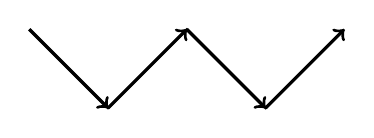
\begin{tikzpicture}
		% define point
		\coordinate (A)  at (1, 1);
		\coordinate (O)  at (2, 0);
		\coordinate (B)  at (3, 1);
		\coordinate (C)  at  (4,0);
		\coordinate (D) at  (5,1);
		% angle  
		\draw[thick] (A) -- (O) -- (B) -- (C)-- (D);
		\draw [->, very thick] (1,1) -- (2,0)  node [midway, above] {\scriptsize };
		\draw [->, very thick] (2,0) -- (3,1)  node [midway, above] {\scriptsize };
		\draw [->, very thick] (3,1) -- (4,0)  node [midway, above] {\scriptsize };
		\draw [->, very thick] (4,0) -- (5,1)  node [midway, above] {\scriptsize };
	\end{tikzpicture}
	\captionof{figure}{\textbf{Wing Gesture}}
	\label{Fig:5.9}
\end{center}

\begin{figure}[H]\centering
	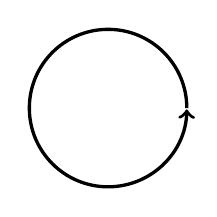
\begin{tikzpicture}
		\draw[->,very thick] (0,0) arc[radius=1cm,start angle=0,delta angle=359];
	\end{tikzpicture}
	\captionof{figure}{\textbf{Ring Gesture }}
	\label{Fig:5.10}
\end{figure}

\begin{figure}[H]\centering
	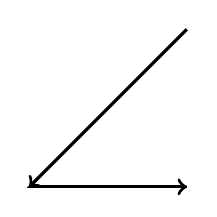
\begin{tikzpicture}
		% define point
		\coordinate (A)  at (2, 2);
		\coordinate (O)  at (0, 0);
		\coordinate (B)  at (2, 0);
		% angle  
		\draw[thick] (A) -- (O) -- (B);
		\draw [->, very thick] (2,2) -- (0,0)  node [midway, above] {\scriptsize };
		\draw [->, very thick] (0,0) -- (2,0)  node [midway, above] {\scriptsize };
	\end{tikzpicture}
	\captionof{figure}{\textbf{Slope Gesture }}
	\label{Fig:5.11}
\end{figure}

\subsection{Regression}

In a regression task, the CNN output is a continuous numerical value. The network is designed to predict a specific numerical outcome, and the final layer often uses an activation function, such as linear, that allows for unbounded output. The training process involves minimizing the difference between the predicted value and the actual target value, as determined by the chosen loss function \cite{Xu:2022}.

\subsection{Output of the Model for Magic Wand}
\label{subsection:outputCNN}

The CNN functions as a classifier, producing class probabilities as its output. The final outcome is determined by the softmax layer \ref{Softmax Function}, resulting in a set of numerical values corresponding to different gesture categories. For example, if the magic wand project involves recognizing gestures like "swirl," "tap," "circle," and "wave," the model might output probabilities such as \texttt{[0.05, 0.70, 0.10, 0.15]}.

Each number in the output array represents the model's confidence score for a specific gesture category, and the category with the highest score is considered the model's prediction for the given input gesture. In the provided example, the model predicts that the gesture category "tap" is the most likely result with a confidence score of 0.70.

To enhance the reliability of gesture recognition, postprocessing techniques can be applied. Methods like score averaging or consensus-based recognition are commonly used. Averaging scores over multiple runs contributes to a more stable and consistent output, improving the model's ability to adapt to variations in gesture patterns and environmental conditions \cite{Warden:2020}.

Upon successful recognition of a gesture, the magic wand's command responder can utilize the device's output capabilities, triggering actions such as changing LED colors, producing sounds, or initiating specific functions. The two-dimensional structure of the model's output, aligning with the first dimension as a wrapper and the second holding probabilities for each gesture class, is designed to suit the requirements of the embedded hardware implementation on Arduino Nano 33 BLE Sense \cite{Zhu:2019}.

\subsubsection{The Softmax Function}
\label{Softmax Function}
The softmax function is commonly used in Convolutional Neural Networks (CNNs) and other machine learning models, particularly in the output layer, to convert a vector of raw scores or logits into probabilities. It essentially normalizes the input values into a probability distribution that sums to 1 \cite{Sewak:2018}.

In the context of CNNs, the softmax function is often applied to the output layer when the network is used for classification tasks. Here's the formula for the softmax function:

\begin{equation}
	\text{Softmax}(x_i) = \frac{e^{x_i}}{\sum_{j=1}^{K} e^{x_j}}
\end{equation}

Where \( x_i \) is the raw score or logit for class \( i \), \( K \) is the total number of classes, and \( e \) is the base of the natural logarithm (Euler's number). An example of applying the Softmax function is shown in Figure \ref{fig:softmax}.

\begin{figure}[h!]
	\centering
	\includegraphics[width=0.4\textwidth]{Images/Algorithm/softmax}
	\caption{Example of applying the softmax function \cite{Sewak:2018}} \label{fig:softmax}
\end{figure}

\section{Python Example Code}
\label{section:AlgorithmExampleCode}


The identification of regional patterns within an image is facilitated by the convolutional layer. Following the convolutional layer, the max pooling layer is employed to diminish dimensionality. This section illustrates image classification by using a code provided by Sewak et al \cite{Sewak:2018}.

It is crucial to initially standardize all images to a uniform size. The initial convolution layer necessitates an additional parameter, \PYTHON{input.shape()}. The focus here is on training a Convolutional Neural Network (CNN) for image classification using the CIFAR-10 database. CIFAR-10 comprises 60,000 color images, each of size $32 \times 32$. These images are categorized into 10 classes, with 6,000 images per category, namely airplane, automobile, bird, cat, dog, deer, frog, horse, ship, and truck.

\subsection{Imports}

In the Listing \ref{code:cnnImports} are the necessary libraries and modules required for working with neural networks, image data, and visualization. The versions are shown in the Table \ref{tab:cnnlibraryVersions}.

\begin{itemize}
	\item Python version: 3.9.
\end{itemize}

\begin{table}[htbp]
	\centering
	\caption{Versions of Libraries}
	\label{tab:cnnlibraryVersions}
	\begin{tabular}{|l|c|}
		\hline
		\textbf{Library} & \textbf{Version} \\
		\hline
		Numpy & 1.23.5 \\
		Matplotlib & 3.7.1 \\
		Keras & 2.12.0 \\
		\hline
	\end{tabular}
\end{table}

\begin{code}[h!]
	\lstinputlisting[style=pythonstyle, numbers=none, linerange={82-89}]{Code/CNN/CNNDataMining.py}    
	\caption{Importing necessary libraries and modules.}
	\label{code:cnnImports}
\end{code}


\subsection{Load CIFAR-10 Dataset}

In Listing \ref{code:cnnLoadCifar} the CIFAR-10 dataset is loaded.CIFAR-10 is a dataset of 50,000 $32 \times 32$ color training images and 10,000 test images.

\begin{code}[h!]
	\lstinputlisting[style=pythonstyle, numbers=none, linerange={107-107}]{Code/CNN/CNNDataMining.py}    
	\caption{Loading and preparing the CIFAR-10 dataset.}
	\label{code:cnnLoadCifar}
\end{code}

\subsubsection{Data Preprocessing}

In the Listing \ref{code:cnnDataPreprocessing} the image data is normalized and one-hot encoding is performed on the labels. The training set is split into training and validation sets.

\begin{code}[h!]
	\lstinputlisting[style=pythonstyle, numbers=none, linerange={124-133}]{Code/CNN/CNNDataMining.py}    
	\caption{Preprocessing data: normalization, one-hot encoding, and splitting into training and validation sets}
	\label{code:cnnDataPreprocessing}
\end{code}

\subsection{Augmented Image Generator}

In the Listing \ref{code:cnnAugmentedGenerator} image data generators for training and validation is created and configured. These generators will perform data augmentation, such as shifting and flipping, to increase the diversity of the training set.

\begin{code}[h!]
	\lstinputlisting[style=pythonstyle, numbers=none, linerange={154-168}]{Code/CNN/CNNDataMining.py}    
	\caption{Configuring image data generators for augmentation and fitting them on training and validation data}
	\label{code:cnnAugmentedGenerator}
\end{code}

\subsection{Plot the First Nine Images of Cifar-10}

Listing \ref{code:cnnPlotCifar10} loads the cifar-10 dataset and plots the first nine images as shown in Figure \ref{fig:cnnFirstNineCifar10}.

\begin{code}[h!]
	\lstinputlisting[style=pythonstyle, numbers=none, linerange={177-183}]{Code/CNN/CNNDataMining.py}    
	\caption{Loading and visualizing the first nine images from the CIFAR-10 dataset}
	\label{code:cnnPlotCifar10}
\end{code}


\begin{figure}[h!]
	\centering
	\includegraphics[width=0.8\textwidth]{Images/Algorithm/CIFAR10SecondNineImages}
	\caption{First nine images from the CIFAR-10 dataset.} \label{fig:cnnFirstNineCifar10}
\end{figure}

\subsection{CNN Model Definition}

A Convolutional Neural Network (CNN) model is defined in Listing \ref{code:cnnDefinition} using Keras with convolutional layers, max pooling, dropout for regularization, and dense layers.

\begin{code}[h!]
	\lstinputlisting[style=pythonstyle, numbers=none, linerange={199-207}]{Code/CNN/CNNDataMining.py}    
	\caption{Defining a Convolutional Neural Network (CNN) model using Keras}
	\label{code:cnnDefinition}
\end{code}

\subsection{Compile the Model}

In Listing \ref{code:cnnCompileModel} the model is compiled with the specified loss function, optimizer, and evaluation metric.

\begin{code}[h!]
	\lstinputlisting[style=pythonstyle, numbers=none, linerange={223-223}]{Code/CNN/CNNDataMining.py}    
	\caption{Compiling the CNN model with specified loss function, optimizer, and metric}
	\label{code:cnnCompileModel}
\end{code}

\subsection{Train the Model with Augmented Data}

In Listing \ref{code:cnnTrainAugmented} the model is trained using the augmented data generators. This involves calling the \PYTHON{fit\_generator} function instead of \PYTHON{fit} and providing the data generators for training and validation sets.

\begin{code}[h!]
	\lstinputlisting[style=pythonstyle, numbers=none, linerange={238-247}]{Code/CNN/CNNDataMining.py}    
	\caption{Training the CNN model with augmented data using data generators}
	\label{code:cnnTrainAugmented}
\end{code}


\subsection{Plotting the Loss and Accuracy Curves}

In Listing \ref{code:cnnLossAccuracyPlot} the accuracy and loss curves are plotted. The results are shown in the Figure \ref{fig:AccuracyandLoss}. The observed trends in the training and validation metrics, with a downward trend in both training and validation loss and an upward trend in accuracy, indicate positive learning and generalization behavior of the neural network. The somewhat unconventional scenario of validation loss being below training loss and validation accuracy exceeding training accuracy could be influenced by effective data augmentation, contributing to the model's robustness. These trends collectively suggest that the model is not overfitting the training data and is likely to generalize well to unseen data, highlighting successful training and potential for further improvement.

\begin{code}[h!]
	\lstinputlisting[style=pythonstyle, numbers=none, linerange={263-284}]{Code/CNN/CNNDataMining.py}    
	\caption{Plotting the loss and accuracy curves}
	\label{code:cnnLossAccuracyPlot}
\end{code}

\begin{figure}[h!]
	\centering
	
	\begin{subfigure}{0.45\textwidth}
		\includegraphics[width=\linewidth]{Images/Algorithm/lossPlot}
		\caption{}    % \caption{} is kept to keep (a), (b), (c) etc. below each subfigure.
		\label{subfig:lossTrends}
	\end{subfigure}
	\hfill
	\begin{subfigure}{0.45\textwidth}
		\includegraphics[width=\linewidth]{Images/Algorithm/accuracyPlot}
		\caption{}    % \caption{} is kept to keep (a), (b), (c) etc. below each subfigure.
		\label{subfig:accuracyTrends}
	\end{subfigure}
	
	\caption{(\subref{subfig:DigitalImage}) Training and validation loss trends over epochs. (\subref{subfig:DigitalImagePixelValues}) Training and validation accuracy trends over epochs.}
	\label{fig:AccuracyandLoss}
\end{figure}

